\section{Introduction}

Dans le cadre de ma formation d'ingénieur à l'\emph{École Nationale Supérieure d'électricité et de Mécanique}, j'ai réalisé un stage du 2 février 2017 au 2 août 2017 au sein du laboratoire ThereSIS de THALES Services à Palaiseau, dans le campus de Saclay. J'ai eu l'occasion pendant ce stage d'effectuer de nombreux séjours à l'INRIA Tao pendant lesquels j'ai pu m'entretenir avec des chercheurs en apprentissage par renforcement et me tenir au courant des avancées dans le domaine de l'intelligence artificielle.

J'ai réalisé ce stage au sein de l'équipe AS&BSIM (Adaptative Systems and
Biomimetic Simulation), qui travaille principalement sur le logiciel \textbf{SE-STAR}. Il s’agit d’un environnement synthétique où évoluent de nombreux agents virtuels, chacun disposant d’un modèle cognitif. 

Dans le cadre de ces simulations, je me suis intéressé à la navigation d'un agent en utilisant l'apprentissage par renforcement profond pour contrôler l'agent dans son environnement. En particulier, la contrainte imposée sur le contrôle de l'agent est qu'en entrée du contrôleur, nous n'avions accès qu'à une image 2D d'un environnement 3D (en l'occurrence SE-STAR).



\subsection{Contexte du stage et de l'entreprise}

Le groupe THALES est une multinationale française employant 67 000 salariés
dans 56 pays. Si l’entreprise est connue auprès du grand public pour sa présence
sur le marché de la défense, elle opère aussi sur plusieurs marchés duaux (à la
fois civils et militaires) : l’aéronautique, l’espace et la sécurité, ainsi que sur le
marché civil du transport terrestre. Les problématiques de traitement et
interprétation des données ainsi que d’aide à la prise de décision sont au cœur
de l’activité du groupe. Afin de renforcer la position du groupe dans l’innovation
autour des nouvelles technologies, les activités de recherche et développement
sont au cœur de l’entreprise, représentant 20\% de ses revenus. THALES possède
un réseau international de laboratoires qui coopèrent avec des universités et des
laboratoires de recherche publics.

THALES Services est une division de THALES, dont l’activité se situe autour des
systèmes d’information et de communications sécurisés.
ThereSIS (THALES European Research for E-Government & Secured Information
Systems) est le laboratoire de recherche en systèmes d’information de THALES
Services. Il est situé sur le site de THALES Research and Technology à Palaiseau.
Les équipes en place ont pour mission de tester des technologies
innovantes, afin de déterminer si elles peuvent être exploitées au profit du
groupe THALES et de ses clients. Des démonstrateurs sont mis en place pour
présenter aux clients des cas concrets d’utilisation de ces technologies
novatrices, parmi lesquelles on peut trouver le cloud computing, les systèmes de
vidéosurveillances, les simulateurs.

Depuis quelques années, ThereSIS a mis l'accent sur les technologies autour de l'intelligence artificielle, et propose une expertise dans ce domaine. Cela permet à THALES d'être un acteur de poids dans les domaines de de la cybersécurité et de la sécurité des infrastructures critiques (gares, aéroports, ...).

ThereSIS propose des projets de recherche ou répond à des appels d’offres
émanant d’entreprises ou de groupes finançant la recherche industrielle. L’intérêt
des clients pour les prototypes présentés peut mener à une phase
d’industrialisation et de commercialisation prise en charge par les départements
de production de THALES Services.

\bigskip
En quelques chiffres, voici une vue de la taille de THALES et de l'importance donnée à la R&D: 
\bigskip
\begin{figure}[!h]
\centering
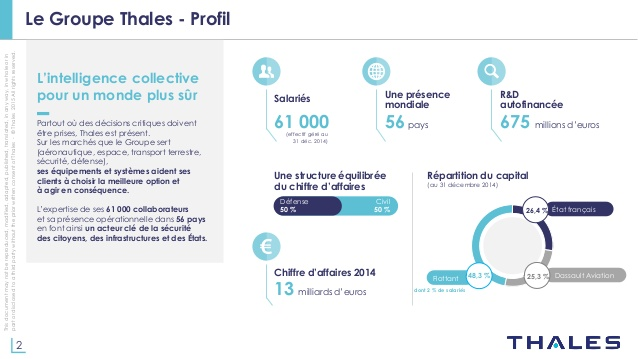
\includegraphics[width=.9\linewidth]{./assets/thales_chiffres}
\caption{THALES en quelques chiffres}
\medskip
\small
\end{figure}
